\PassOptionsToPackage{unicode=true}{hyperref} % options for packages loaded elsewhere
\PassOptionsToPackage{hyphens}{url}
%
\documentclass[]{article}
\usepackage{lmodern}
\usepackage{amssymb,amsmath}
\usepackage{ifxetex,ifluatex}
\usepackage{fixltx2e} % provides \textsubscript
\ifnum 0\ifxetex 1\fi\ifluatex 1\fi=0 % if pdftex
  \usepackage[T1]{fontenc}
  \usepackage[utf8]{inputenc}
  \usepackage{textcomp} % provides euro and other symbols
\else % if luatex or xelatex
  \usepackage{unicode-math}
  \defaultfontfeatures{Ligatures=TeX,Scale=MatchLowercase}
\fi
% use upquote if available, for straight quotes in verbatim environments
\IfFileExists{upquote.sty}{\usepackage{upquote}}{}
% use microtype if available
\IfFileExists{microtype.sty}{%
\usepackage[]{microtype}
\UseMicrotypeSet[protrusion]{basicmath} % disable protrusion for tt fonts
}{}
\IfFileExists{parskip.sty}{%
\usepackage{parskip}
}{% else
\setlength{\parindent}{0pt}
\setlength{\parskip}{6pt plus 2pt minus 1pt}
}
\usepackage{hyperref}
\hypersetup{
            pdfborder={0 0 0},
            breaklinks=true}
\urlstyle{same}  % don't use monospace font for urls
\usepackage[margin=1in]{geometry}
\usepackage{color}
\usepackage{fancyvrb}
\newcommand{\VerbBar}{|}
\newcommand{\VERB}{\Verb[commandchars=\\\{\}]}
\DefineVerbatimEnvironment{Highlighting}{Verbatim}{commandchars=\\\{\}}
% Add ',fontsize=\small' for more characters per line
\usepackage{framed}
\definecolor{shadecolor}{RGB}{248,248,248}
\newenvironment{Shaded}{\begin{snugshade}}{\end{snugshade}}
\newcommand{\AlertTok}[1]{\textcolor[rgb]{0.94,0.16,0.16}{#1}}
\newcommand{\AnnotationTok}[1]{\textcolor[rgb]{0.56,0.35,0.01}{\textbf{\textit{#1}}}}
\newcommand{\AttributeTok}[1]{\textcolor[rgb]{0.77,0.63,0.00}{#1}}
\newcommand{\BaseNTok}[1]{\textcolor[rgb]{0.00,0.00,0.81}{#1}}
\newcommand{\BuiltInTok}[1]{#1}
\newcommand{\CharTok}[1]{\textcolor[rgb]{0.31,0.60,0.02}{#1}}
\newcommand{\CommentTok}[1]{\textcolor[rgb]{0.56,0.35,0.01}{\textit{#1}}}
\newcommand{\CommentVarTok}[1]{\textcolor[rgb]{0.56,0.35,0.01}{\textbf{\textit{#1}}}}
\newcommand{\ConstantTok}[1]{\textcolor[rgb]{0.00,0.00,0.00}{#1}}
\newcommand{\ControlFlowTok}[1]{\textcolor[rgb]{0.13,0.29,0.53}{\textbf{#1}}}
\newcommand{\DataTypeTok}[1]{\textcolor[rgb]{0.13,0.29,0.53}{#1}}
\newcommand{\DecValTok}[1]{\textcolor[rgb]{0.00,0.00,0.81}{#1}}
\newcommand{\DocumentationTok}[1]{\textcolor[rgb]{0.56,0.35,0.01}{\textbf{\textit{#1}}}}
\newcommand{\ErrorTok}[1]{\textcolor[rgb]{0.64,0.00,0.00}{\textbf{#1}}}
\newcommand{\ExtensionTok}[1]{#1}
\newcommand{\FloatTok}[1]{\textcolor[rgb]{0.00,0.00,0.81}{#1}}
\newcommand{\FunctionTok}[1]{\textcolor[rgb]{0.00,0.00,0.00}{#1}}
\newcommand{\ImportTok}[1]{#1}
\newcommand{\InformationTok}[1]{\textcolor[rgb]{0.56,0.35,0.01}{\textbf{\textit{#1}}}}
\newcommand{\KeywordTok}[1]{\textcolor[rgb]{0.13,0.29,0.53}{\textbf{#1}}}
\newcommand{\NormalTok}[1]{#1}
\newcommand{\OperatorTok}[1]{\textcolor[rgb]{0.81,0.36,0.00}{\textbf{#1}}}
\newcommand{\OtherTok}[1]{\textcolor[rgb]{0.56,0.35,0.01}{#1}}
\newcommand{\PreprocessorTok}[1]{\textcolor[rgb]{0.56,0.35,0.01}{\textit{#1}}}
\newcommand{\RegionMarkerTok}[1]{#1}
\newcommand{\SpecialCharTok}[1]{\textcolor[rgb]{0.00,0.00,0.00}{#1}}
\newcommand{\SpecialStringTok}[1]{\textcolor[rgb]{0.31,0.60,0.02}{#1}}
\newcommand{\StringTok}[1]{\textcolor[rgb]{0.31,0.60,0.02}{#1}}
\newcommand{\VariableTok}[1]{\textcolor[rgb]{0.00,0.00,0.00}{#1}}
\newcommand{\VerbatimStringTok}[1]{\textcolor[rgb]{0.31,0.60,0.02}{#1}}
\newcommand{\WarningTok}[1]{\textcolor[rgb]{0.56,0.35,0.01}{\textbf{\textit{#1}}}}
\usepackage{longtable,booktabs}
% Fix footnotes in tables (requires footnote package)
\IfFileExists{footnote.sty}{\usepackage{footnote}\makesavenoteenv{longtable}}{}
\usepackage{graphicx,grffile}
\makeatletter
\def\maxwidth{\ifdim\Gin@nat@width>\linewidth\linewidth\else\Gin@nat@width\fi}
\def\maxheight{\ifdim\Gin@nat@height>\textheight\textheight\else\Gin@nat@height\fi}
\makeatother
% Scale images if necessary, so that they will not overflow the page
% margins by default, and it is still possible to overwrite the defaults
% using explicit options in \includegraphics[width, height, ...]{}
\setkeys{Gin}{width=\maxwidth,height=\maxheight,keepaspectratio}
\setlength{\emergencystretch}{3em}  % prevent overfull lines
\providecommand{\tightlist}{%
  \setlength{\itemsep}{0pt}\setlength{\parskip}{0pt}}
\setcounter{secnumdepth}{5}
% Redefines (sub)paragraphs to behave more like sections
\ifx\paragraph\undefined\else
\let\oldparagraph\paragraph
\renewcommand{\paragraph}[1]{\oldparagraph{#1}\mbox{}}
\fi
\ifx\subparagraph\undefined\else
\let\oldsubparagraph\subparagraph
\renewcommand{\subparagraph}[1]{\oldsubparagraph{#1}\mbox{}}
\fi

% set default figure placement to htbp
\makeatletter
\def\fps@figure{htbp}
\makeatother

\usepackage{booktabs}
\usepackage{amsthm}
\makeatletter
\def\thm@space@setup{%
  \thm@preskip=8pt plus 2pt minus 4pt
  \thm@postskip=\thm@preskip
}
\makeatother

\newenvironment{rmdattachment}
  {\begin{center}}
  {\end{center}}

\newenvironment{rmdwebsite}
  {\begin{center}}
  {\end{center}}
  
\newenvironment{rmdblankbox}
  {\begin{center}}
  {\end{center}}
\usepackage[]{natbib}
\bibliographystyle{plainnat}

\author{}
\date{\vspace{-2.5em}}

\begin{document}

{
\setcounter{tocdepth}{2}
\tableofcontents
}
\hypertarget{part-session-1}{%
\part{Session 1}\label{part-session-1}}

\hypertarget{session_01_01}{%
\section{Getting started - Project Setup}\label{session_01_01}}

\hypertarget{installing-r-rstudio-ide}{%
\subsection{ Installing R \& RStudio IDE}\label{installing-r-rstudio-ide}}

\hypertarget{interactively}{%
\subsubsection{Interactively}\label{interactively}}

Go to the following link and follow the instructions to install R and the IDE RStudio

\begin{rmdblankbox}
Interactive Shinyapp
\end{rmdblankbox}
\begin{rmdshiny}
Install R \& RStudio IDE
\end{rmdshiny}

\hypertarget{manually}{%
\subsubsection{Manually}\label{manually}}

\textbf{Video instructions to install RStudio (Download link below)}

\begin{rmdblankbox}
Download
\end{rmdblankbox}
\begin{rmdattachment}
\textbf{\url{https://cloud.r-project.org}}
\end{rmdattachment}

\begin{center}\rule{0.5\linewidth}{0.5pt}\end{center}

\textbf{Video instructions to install RStudio (Download link below)}

\begin{rmdblankbox}
Download
\end{rmdblankbox}
\begin{rmdattachment}
\textbf{\url{https://rstudio.com/products/rstudio/download/}}
\end{rmdattachment}

\begin{center}\rule{0.5\linewidth}{0.5pt}\end{center}

\textbf{Video instructions to install R packages}

Installing Packages

\begin{Shaded}
\begin{Highlighting}[]
\CommentTok{# install package from CRAN}
\KeywordTok{install.packages}\NormalTok{(}\StringTok{"dplyr"}\NormalTok{)   }
\end{Highlighting}
\end{Shaded}

Loading packages

\begin{Shaded}
\begin{Highlighting}[]
\CommentTok{# load the package to use in the current R session}
\KeywordTok{library}\NormalTok{(}\StringTok{"packagename"}\NormalTok{)         }

\CommentTok{# use a particular function within a package without loading the package}
\NormalTok{packagename}\OperatorTok{::}\NormalTok{functionname   }
\end{Highlighting}
\end{Shaded}

\hypertarget{running-r-code-stolen-from-r4ds}{%
\subsection{ Running R code (stolen from R4DS)}\label{running-r-code-stolen-from-r4ds}}

The previous section showed you a couple of examples of running R code. Code in the book looks like this:

\begin{verbatim}
1 + 2
## [1] 3
\end{verbatim}

If you run the same code in your local console, it will look like this:

\begin{verbatim}
> 1 + 2
[1] 3
\end{verbatim}

There are two main differences. In your console, you type after the \texttt{\textgreater{}}, called the \textbf{prompt}; we don't show the prompt in the book. In the book, output is commented out with \texttt{\#\textgreater{}}; in your console it appears directly after your code. These two differences mean that if you're working with an electronic version of the book, you can easily copy code out of the book and into the console.
Throughout the book we use a consistent set of conventions to refer to code:
* Functions are in a code font and followed by parentheses, like \texttt{sum()},
or \texttt{mean()}.
* Other R objects (like data or function arguments) are in a code font,
without parentheses, like \texttt{flights} or \texttt{x}.

\begin{itemize}
\tightlist
\item
  If we want to make it clear what package an object comes from, we'll use
  the package name followed by two colons, like \texttt{dplyr::mutate()}, or\\
  \texttt{nycflights13::flights}. This is also valid R code.
\end{itemize}

\hypertarget{exercise-1}{%
\subsection{ Exercise 1}\label{exercise-1}}

\begin{enumerate}
\def\labelenumi{\arabic{enumi}.}
\tightlist
\item
  Identify what working directory you are working out of.
\item
  Create a folder on your computer titled \texttt{datascience}. Within R, set your working directory to this folder.
\end{enumerate}

\hypertarget{solution}{%
\subsubsection*{Solution}\label{solution}}
\addcontentsline{toc}{subsubsection}{Solution}

\begin{enumerate}
\def\labelenumi{\arabic{enumi}.}
\tightlist
\item
  Identify what working directory you are working out of.
\end{enumerate}

\begin{Shaded}
\begin{Highlighting}[]
\KeywordTok{getwd}\NormalTok{()}
\CommentTok{#> [1] "/Users/j.schwarz/NIT/"}
\end{Highlighting}
\end{Shaded}

\begin{enumerate}
\def\labelenumi{\arabic{enumi}.}
\setcounter{enumi}{1}
\tightlist
\item
  Create a folder on your computer titled \texttt{datascience}. Within R, set your working directory to this folder.
\end{enumerate}

\begin{Shaded}
\begin{Highlighting}[]
\KeywordTok{setwd}\NormalTok{(}\StringTok{"/Users/j.schwarz/NIT/datascience"}\NormalTok{)}
\end{Highlighting}
\end{Shaded}

\hypertarget{exercise-2}{%
\subsection{ Exercise 2}\label{exercise-2}}

\texttt{dplyr} is an extremely popular package for common data transformation activities and is available from CRAN. Perform the following tasks:

\begin{enumerate}
\def\labelenumi{\arabic{enumi}.}
\tightlist
\item
  Install the \texttt{dplyr} package.
\item
  Load the \texttt{dplyr} package.
\item
  Access the help documentation for the \texttt{dplyr} package.
\item
  Check out the vignette(s) for \texttt{dplyr}
\end{enumerate}

\hypertarget{solution-1}{%
\subsubsection*{Solution}\label{solution-1}}
\addcontentsline{toc}{subsubsection}{Solution}

\begin{enumerate}
\def\labelenumi{\arabic{enumi}.}
\tightlist
\item
  Install the \texttt{tidyverse} package.
\end{enumerate}

\begin{Shaded}
\begin{Highlighting}[]
\KeywordTok{install.packages}\NormalTok{(}\StringTok{"tidyverse"}\NormalTok{)}
\end{Highlighting}
\end{Shaded}

\begin{enumerate}
\def\labelenumi{\arabic{enumi}.}
\setcounter{enumi}{1}
\tightlist
\item
  Load the \texttt{tidyverse} package.
\end{enumerate}

\begin{Shaded}
\begin{Highlighting}[]
\KeywordTok{library}\NormalTok{(tidyverse)}
\end{Highlighting}
\end{Shaded}

\begin{verbatim}
## -- Attaching packages -------------------------------------------------------------------------------------- tidyverse 1.3.0 --
\end{verbatim}

\begin{verbatim}
## v ggplot2 3.2.1     v purrr   0.3.3
## v tibble  2.1.3     v dplyr   0.8.3
## v tidyr   1.0.2     v stringr 1.4.0
## v readr   1.3.1     v forcats 0.4.0
\end{verbatim}

\begin{verbatim}
## -- Conflicts ----------------------------------------------------------------------------------------- tidyverse_conflicts() --
## x dplyr::filter() masks stats::filter()
## x dplyr::lag()    masks stats::lag()
\end{verbatim}

\hypertarget{working-with-rstudio-setup-customization}{%
\subsection{Working with RStudio / Setup \& Customization}\label{working-with-rstudio-setup-customization}}

\hypertarget{console}{%
\subsubsection{Console}\label{console}}

\hypertarget{script-editor}{%
\subsubsection{Script Editor}\label{script-editor}}

\hypertarget{workspace-environment}{%
\subsubsection{Workspace Environment}\label{workspace-environment}}

\hypertarget{misc.-displays}{%
\subsubsection{Misc. Displays}\label{misc.-displays}}

\hypertarget{getting-started-with-github}{%
\section{Getting started with github}\label{getting-started-with-github}}

\begin{enumerate}
\def\labelenumi{\arabic{enumi}.}
\tightlist
\item
  Create a free github account.
\end{enumerate}

\begin{rmdblankbox}
Website
\end{rmdblankbox}
\begin{rmdwebsite}
\textbf{\url{https://github.com/}}
\end{rmdwebsite}

\begin{enumerate}
\def\labelenumi{\arabic{enumi}.}
\setcounter{enumi}{1}
\tightlist
\item
  Download and install github desktop
\end{enumerate}

\begin{rmdblankbox}
Download
\end{rmdblankbox}
\begin{rmdattachment}
\textbf{\url{https://desktop.github.com}}
\end{rmdattachment}

\hypertarget{setting-up-the-project}{%
\section{Setting Up The Project}\label{setting-up-the-project}}

\begin{rmdblankbox}
Download
\end{rmdblankbox}
\begin{rmdattachment}
\textbf{\href{https://github.com/TUHH-W11/data-science/blob/master/files/session_01/business_case_01.zip}{business\_case\_01.zip}}
\end{rmdattachment}

\begin{figure}
\centering
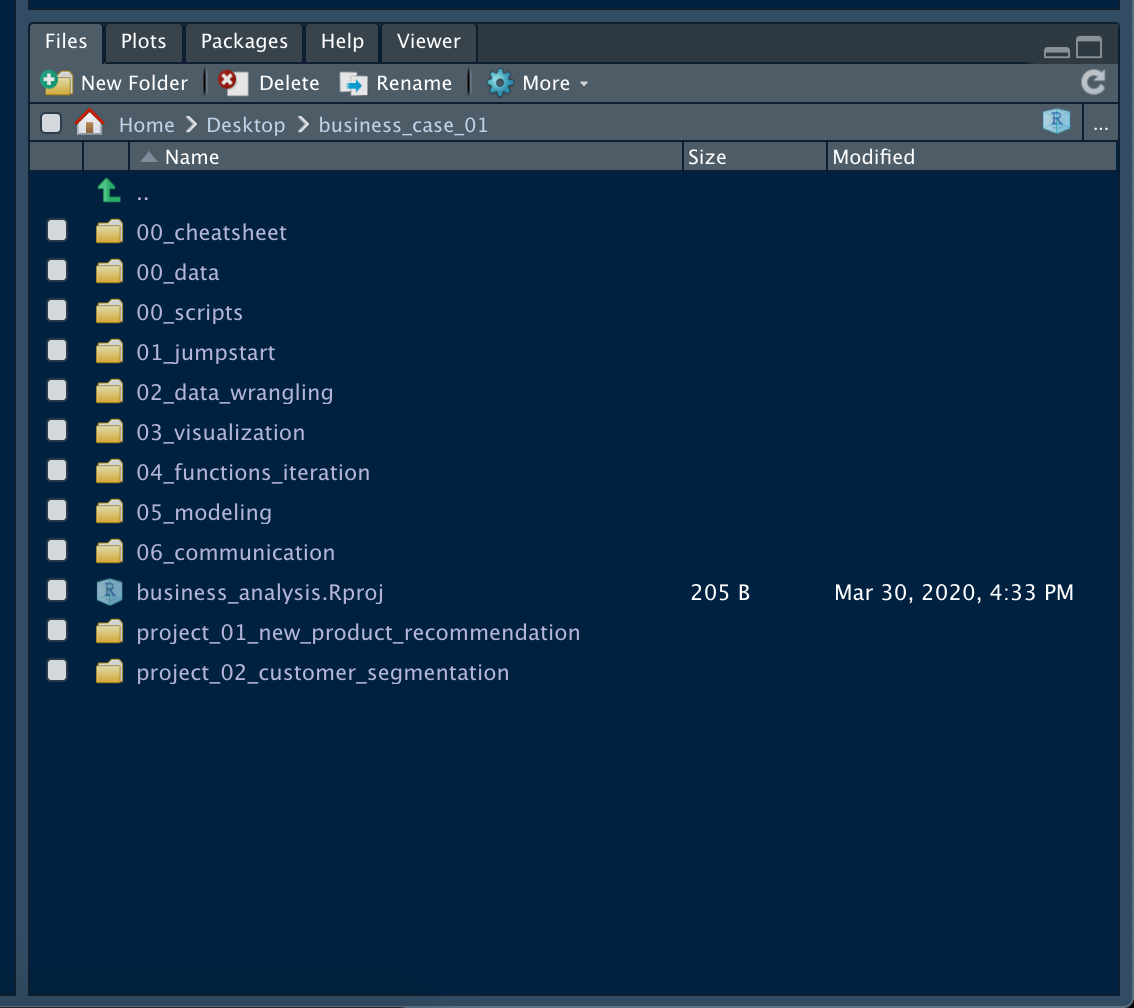
\includegraphics{input/images/session_01/project_structure.png}
\caption{project structure}
\end{figure}

\end{document}
